% !TEX encoding = UTF-8 Unicode
% !TEX program = lualatexmk
% !TEX pdfSinglePage
\documentclass[12pt]{article}
%% Versioning info
%\usepackage[draft]{gitinfo2}
%% Polices OTF
\usepackage[libertine,libaltvw,liby,vvarbb]{newtxmath}
\usepackage[ttscale=.875]{libertine}
%\setmainfont{Lucida Grande}
%% Gestion des langues
\usepackage{polyglossia}
\setdefaultlanguage{english}
\usepackage[autostyle]{csquotes}
\MakeOuterQuote{"}
%% URLs and hyperlinks
\usepackage{xcolor}
\usepackage[unicode,bookmarks,colorlinks,breaklinks]{hyperref}
\hypersetup{linkcolor=blue,citecolor=blue,filecolor=blue,urlcolor=blue}
\urlstyle{same}
\usepackage[shortlabels]{enumitem}
\setlist[enumerate,1]{label=\arabic*.,ref=\arabic*,leftmargin=*}
%\setlist[itemize,1]{label=--,topsep=0pt,itemsep=0pt,leftmargin=*}
\setlist[itemize,1]{topsep=0pt,itemsep=0pt,leftmargin=1em}
\setlist[itemize,2]{topsep=0pt,itemsep=0pt}
%% Framed boxes
\usepackage[framemethod=tikz]{mdframed}
\global\mdfdefinestyle{verif}{%
  %linecolor=blue,middlelinewidth=2pt,
  roundcorner=5pt,
  frametitlebackgroundcolor=yellow!50!white,
}
\newmdenv[style=verif,frametitle=Check]{verification}
%% Format de page
\usepackage{geometry}
\geometry{a4paper}
\geometry{top=25mm, bottom=30mm}
\geometry{outer=22.5mm, inner=25mm}
\geometry{foot=15mm, head=15pt}
%% Paragraphes sans indentation, légèrement espacés
\setlength{\parindent}{0pt}
\setlength{\parskip}{3pt plus2pt minus1pt}
%%
\setcounter{tocdepth}{2}
\setcounter{secnumdepth}{1}
%%
\usepackage{listings}
\lstset{%
  basicstyle=\small\ttfamily,breaklines=true,
  showstringspaces=false,
  aboveskip=2\parskip,
  commentstyle=\color{darkgray},
  keywordstyle=\color[HTML]{000000},
  backgroundcolor=\color[HTML]{dddddd},
  tabsize=4,
  xleftmargin=1em,
  framextopmargin=3pt,
  framexleftmargin=1em,
  %framexrightmargin=1em,
  framexbottommargin=2pt,
  frame=bt,
  rulecolor=\color[HTML]{666666},
}
%%
%% Illustrations
\usepackage{graphicx}
\graphicspath{{img/}}

\begin{document}

\title{MoodleBox building reference\\Version 4.8.0%
  \footnote{This work is licensed under a \href{http://creativecommons.org/licenses/by-nc-sa/4.0/}{Creative Commons Attribution - Non Commercial - Share Alike  4.0 International} license.}%
}
\date{\today} %% \footnote{Version \gitAbbrevHash, \gitAuthorDate}
\author{Nicolas Martignoni%
  \footnote{MoodleBox founder and maintainer; teacher in college level mathematics and computer science and teacher trainer in Fribourg, Switzerland.}%
}
\maketitle

\begingroup
\setlength{\parskip}{3pt plus1pt minus1pt}
\tableofcontents
\endgroup
\clearpage

\section{Introduction}

This document explains how to build a MoodleBox manually.
It is intended for developers or system administrators and provide background information on how a MoodleBox is built.
It is not meant to be an end-user documentation.

For the MoodleBox end-user documentation, consult the \href{https://moodlebox.net/}{MoodleBox website}.

The MoodleBox project is a free (as in speech and in beer) and open source project. The Ansible playbook source to build the MoodleBox image is provided under a AGPL v3.0 License. It is available at \href{https://github.com/moodlebox/moodlebox}{GitHub}.

\subsection{Caveat}

The actual build of the MoodleBox image is done automatically using \href{https://www.ansible.com/}{Ansible}.
Using Ansible enables most of the build to be automated, as well as ensuring that it is reproducible.

Though complete, the instructions in this document should not be understood as a method to obtain a MoodleBox that is totally equivalent to the officially published MoodleBox images.

Although the MoodleBox works fine on other Raspberry Pi models, a Raspberry Pi Model 3B, 3B+, 4B or 5 is recommended to \textbf{build} it.

\subsection{What MoodleBox does}

\begin{itemize}
\item Configurable routed wireless access point, with optional captive portal.
\item Internet router: MoodleBox acts as a router and gives its clients access to the Internet, when it is connected via ethernet or wireless LAN to an Internet-connected network.
\item DHCP server for wireless clients.
\item Raspberry Pi Connect:\footnote{\url{https://www.raspberrypi.com/documentation/services/connect.html}.} MoodleBox can be managed from anywhere in the world, when it is connected via ethernet or wireless LAN to an Internet-connected network.
\item Moodle server (\url{http://moodlebox.home/}).
This is a fully standard Moodle installation.
\item MoodleBox plugin\footnote{\url{https://github.com/moodlebox/moodle-tool_moodlebox}.} providing a GUI to manage most aspects of the MoodleBox.
\end{itemize}

\subsubsection{Specific Moodle features}
\begin{itemize}
\item Moodle version 4.5.x in its basic configuration, with no content (no courses).
The only Moodle user account is an administrator account (default username: \emph{moodlebox}, default password: \emph{Moodlebox4\$}).
The server is configured to accept clients from the official Moodle app.\footnote{\url{https://download.moodle.org/mobile/}.}
The \textsl{cron} service is launched every minute.
\item When a USB sticks are inserted into the MoodleBox, their files are available to users in Moodle's \textsl{USB Drives} repository.
\item Ability to upload files via SFTP directly to the MoodleBox; these files are then available to users in Moodle's \textsl{SFTP Documents} repository.
\item AdminerEvo, a full-featured database management tool, is installed (\url{http://moodlebox.home/adminer.php}).
\end{itemize}

\subsection{What MoodleBox doesn't do}

\begin{itemize}
\item Email server: MoodleBox is intended to be used "in the field", independently of any network infrastructure; email server functionality is not relevant for this purpose.
\item Coffee machine.
\end{itemize}

\subsection{Acknowledgements}

MoodleBox uses some of the great ideas from its first proof of concept by Christian Westphal\footnote{Christian Westphal, Académie de Strasbourg, see \url{https://moodle.org/user/view.php?id=1378197&course=20}.}, for which he deserves special thanks.

\section{Preparation of the Raspberry Pi}

\subsection{Copy of Raspberry Pi OS Lite on a microSD card}

For this process, use \href{https://www.raspberrypi.com/software/}{Raspberry Pi Imager}.
A complete description of the process is available on Raspberry Pi web site.\footnote{See \url{https://www.raspberrypi.org/documentation/computers/getting-started.html}.}

Click \textbf{Choose device} and select your Raspberry Pi model from the list.
Next, click \textbf{Choose OS} and select the \emph{Raspberry Pi OS Lite (64-bit)} from the \textbf{Raspberry Pi OS (Other)} list.
Plug then your (good quality!) microSD card with at least 8~GB capacity in your computer, click \textbf{Choose storage} and select your storage device.

Now click \textbf{Edit Settings} button to open OS customisation.
On the \textbf{General} tab, set a hostname, a username and a password.
MoodleBox uses \emph{moodlebox} as a hostname, and the username \emph{moodlebox} and the password \emph{Moodlebox4\$}.
Leave as is all other settings.

On the \textbf{Service} tab, check the box next to \textbf{Enable SSH} and choose the password authentication, then click \textbf{Save} button.
Next, click \textbf{Yes} to apply OS customisation settings when you write the image to the storage device.
Finally, respond \textbf{Yes} to the "Are you sure you want to continue?" popup to begin writing data to the storage device.

When you see the "Write Successful" popup, your image is ready and you may eject it from your computer.

\subsection{First login via SSH}

Insert the microSD card into the Raspberry Pi.

Connect the power supply of the Raspberry Pi.
Plug the Raspberry Pi with an Ethernet cable into a network with a DHCP server and wait 20-30 seconds.
The Raspberry Pi is now reachable on the network using the address \lstinline{moodlebox.local}.\footnote{This network address is provided by the \emph{zeroconf} standard protocol.
Some older Android and Windows devices do not understand this protocol.
With such devices, it is necessary to get access to the Raspberry Pi via its numerical IP address, which must be discovered manually.}

\iffalse
\begin{verification}
Red LED, indicating the presence of power, lights up constantly.
Green LED, indicating accesses to the microSD card, flashes irregularly after 1-2 seconds.
\end{verification}
\fi

\iffalse
\begin{verification}
From a computer, we type the command \lstinline{ping -c3 moodlebox.local}.
The result should be something like the following.

\begin{lstlisting}[language=bash]
$ ping -c3 moodlebox.local
PING moodlebox.local (192.168.1.212): 56 data bytes
64 bytes from 192.168.1.212: icmp_seq=0 ttl=64 time=0.452 ms
64 bytes from 192.168.1.212: icmp_seq=1 ttl=64 time=0.251 ms
64 bytes from 192.168.1.212: icmp_seq=2 ttl=64 time=0.222 ms

--- moodlebox.local ping statistics ---
3 packets transmitted, 3 packets received, 0.0% packet loss
round-trip min/avg/max/stddev = 0.222/0.308/0.452/0.102 ms
\end{lstlisting}
\end{verification}
\fi

From now on, all operations are done via the command line in a regular terminal on macOS and Linux, or with \lstinline{Putty} on Windows.

We can now log in to the Raspberry Pi using the main account we've just setup: username is \emph{moodlebox} with password \emph{Moodlebox4\$}.

\begin{lstlisting}[language=bash]
$ ssh moodlebox@moodlebox.local
$ moodlebox@moodlebox.local's password:
\end{lstlisting}

\iffalse
\begin{verification}
If all goes well, we are connected to the MoodleBox and the console displays

\begin{lstlisting}[language=bash]
The programs included with the Debian GNU/Linux system are free software;
the exact distribution terms for each program are described in the
individual files in /usr/share/doc/*/copyright.

Debian GNU/Linux comes with ABSOLUTELY NO WARRANTY, to the extent
permitted by applicable law.

moodlebox@moodlebox:~ $
\end{lstlisting}
\end{verification}
\fi

\subsection{Raspberry Pi OS upgrade}

We begin by upgrading the Raspberry Pi's operating system and its installed packages, with these commands:
\begin{lstlisting}[language=bash]
$ sudo apt update
$ sudo apt full-upgrade -y
\end{lstlisting}

This step can take several minutes, depending on the available Internet connection speed.
We just wait until it's finished.

\subsection{Fix default user home directory permissions}

We must fix the default user home directory permissions, otherwise certain features will not be available.

\begin{lstlisting}[language=bash]
$ sudo chmod u=rwx,g=rx,o=rx /home/moodlebox/
\end{lstlisting}

\subsection{Configuration of important settings}

Launch \emph{raspi-config} utility:
\begin{lstlisting}[language=bash]
$ sudo raspi-config
\end{lstlisting}

With \emph{raspi-config} utility, we configure the following settings.
\begin{itemize}
\item Expand Filesystem.
\item Install following \emph{locales}:
\begin{itemize}
\item \lstinline{en_GB.UTF-8} (should be already here)
\item \lstinline{en_AU.UTF-8}
\item \lstinline{fr_FR.UTF-8}
\item \lstinline{de_DE.UTF-8}
\item \lstinline{es_ES.UTF-8}
\item \lstinline{it_IT.UTF-8}
\end{itemize}
and set \lstinline{en_GB.UTF-8} as default \emph{locale}.
\item Set time zone and WLAN country.
This will also unblock wireless use.
MoodleBox default settings are respectively \lstinline{Europe/Zurich} and \lstinline{CH}.
\item Set the hostname to \emph{moodlebox}.
\end{itemize}

If hostname is changed, MoodleBox won't work correctly.
To prevent this issue, we check the hostname at first boot and fix it if needed.
This is done by copying the following file to \lstinline{/etc/init.d/fix_hostname_once}, with adequate permissions.

\lstinputlisting{files/fix_hostname_once}

From now on, to connect to the Raspberry Pi (via SSH or SFTP), we'll use the address \lstinline{moodlebox.local}.

Let's reboot and log in to the MoodleBox with the default credentials set up page~\pageref{ssec-new-account}.

\iffalse
\subsection{Raspberry Pi firmware upgrade (optional)}

In very specific and very rare occasions, it's advisable to upgrade the firmware of the Raspberry Pi.
We only do this if we know why, since it could brick the device or the image!
And we reboot immediately.

\begin{lstlisting}[language=bash]
$ sudo apt install -y rpi-update
$ sudo SKIP_BACKUP=1 PRUNE_MODULES=1 rpi-update
$ sudo apt remove rpi-update
$ sudo reboot
\end{lstlisting}
\fi

\subsection{Configuration of the system memory}

To increase the system available memory, we reduce the memory reserved for the graphics chip to 16~MB.
This is of no consequence, as our system does have no graphical interface.
We do this by adding the following line at the end of the file \lstinline{/boot/firmware/config.txt}:
\begin{lstlisting}[language=bash]
gpu_mem=16
\end{lstlisting}

\subsection{Configuration of the shutdown/startup hardware button feature}

We enable shutdown/startup hardware button feature by further editing file \lstinline{/boot/firmware/config.txt}, after \lstinline{# Additional overlays...}, to get:
\begin{lstlisting}[language=bash]
# Additional overlays and parameters are documented
# /boot/firmware/overlays/README
dtoverlay=gpio-shutdown
\end{lstlisting}

\subsection{Limit journald file size to 16~MB}

The \lstinline{journald} log file can become very large.
We limit its size to 16~MB by creating the file \lstinline{/etc/systemd/journald.conf.d/journald_moodlebox.conf}, with the following content:\begin{lstlisting}[language=bash]
[Journal]
SystemMaxUse=16M
\end{lstlisting}

\subsection{Install Raspberry Pi Connect}

Raspberry Pi Connect provides secure access to your Raspberry Pi from anywhere in the world.
We install it so people can manage their MoodleBox from anywhere, provided it is connected to the Internet.
And we reboot before going forward.

\begin{lstlisting}[language=bash]
$ sudo apt install -y rpi-connect-lite
$ sudo loginctl enable-linger
$ sudo reboot
\end{lstlisting}

\section{Wireless access point feature}

We will now setup the wireless access point (AP) of the MoodleBox.

\subsection{Switch to the alternative wireless chip firmware}

The Raspberry Pi is usually used as a wireless client, and its wireless firmware has enhanced client features that are not useful for a MoodleBox, which is mainly used as an access point.

However, the SRAM on the wireless chip is used both for data storage whilst in use, but also for these additional features and for bug fixes.
Each time a feature is added or a bug fix made, the amount of SRAM available for runtime variables decreases, and so the number of clients in access point mode.

An alternative firmware is available that has been tuned to maximise the number of clients in access point mode (AP) while still supporting client mode (STA).

We use this alternative firmware in the MoodleBox.
To switch the firmware to the alternative one, we launch the following command and select \lstinline{cyfmac43455-sdio-minimal.bin} firmware.

\begin{lstlisting}[language=bash]
$ sudo update-alternatives --config cyfmac43455-sdio.bin
\end{lstlisting}

\subsection{Setup of the wireless regulatory country}

We have to set the wireless regulatory country.
MoodleBox default setting for the regulatory country is \lstinline{CH}.
Two steps are required to do this.
We first set it via the \lstinline{iw} utility:
\begin{lstlisting}[language=bash]
$ sudo iw reg set CH
\end{lstlisting}
Then we set it in the kernel command line, by adding \lstinline{cfg80211.ieee80211_regdom=CH} at the end of the unique line of the file \lstinline{/boot/firmware/cmdline.txt}.

\subsection{Configuration of the wireless interface for access point mode}

We want to be able to use standard wireless interface \lstinline{wlan0} to optionally connect to a wireless LAN, so we need another interface for our AP.

We use a \textsl{udev} rule to define this new interface named \lstinline{uap0}, creating a file named \lstinline{90-wireless.rules} in directory \lstinline{/etc/udev/rules.d/}.

Here's the content of \lstinline{/etc/udev/rules.d/90-wireless.rules} on the MoodleBox:
\lstinputlisting{files/90-wireless.rules}

\subsection{Configuration of the static IP address}\label{ssec-static-ip}

MoodleBox gets dynamically via DHCP its IP address on the ethernet interface \lstinline{eth0} or as a wireless client on the \lstinline{wlan0} interface.

With its routed access point feature, it will also act as a DHCP provider on its wireless interface \lstinline{uap0}, so we need a static IP address on \lstinline{uap0} interface.

We edit now the file \lstinline{/etc/hosts}, replacing the last line, beginning with \lstinline{127.0.1.1}, with the following, containing the static IP address.
For the MoodleBox, the static IP address chosen is \lstinline{10.0.0.1}.
Any other private IP address can alternatively be used.
\begin{lstlisting}[language=bash]
10.0.0.1	moodlebox
\end{lstlisting}
%This configuration enables any device to access the MoodleBox via its URL \url{http://moodlebox.home/}, even those that do not implement \emph{zeroconf}\footnote{\url{https://en.wikipedia.org/wiki/Zero-configuration_networking}} standard protocol.

\subsection{Configuration of the access point}

We create the wifi access point connection using NetworkManager.
Note we use the interface \lstinline{uap0} and the static IP address we just defined.
Other settings such as SSID, password and wireless channel can be changed.
\begin{lstlisting}[language=bash]
$ sudo nmcli c add type wifi ifname uap0 con-name WifiAP ssid MoodleBox
$ sudo nmcli c mod WifiAP autoconnect yes 802-11-wireless.mode ap \
    802-11-wireless.band bg 802-11-wireless.channel 11
$ sudo nmcli c mod WifiAP ipv4.address 10.0.0.1/24 ipv4.gateway 10.0.0.1 \
    ipv4.method shared
$ sudo nmcli c mod WifiAP wifi-sec.key-mgmt wpa-psk wifi-sec.psk moodlebox
$ sudo nmcli c mod WifiAP wifi-sec.proto rsn wifi-sec.group ccmp \
    wifi-sec.pairwise ccmp
\end{lstlisting}

We change some settings of the AP, in particular the DHCP settings, by adding a configuration file to \lstinline{dnsmasq} instance managed by NetworkManager.
The file has to be placed in \lstinline{/etc/NetworkManager/dnsmasq-shared.d/}
Here's the content of MoodleBox setting file \lstinline{/etc/NetworkManager/dnsmasq-shared.d/00-dhcp.conf}:
\lstinputlisting{files/00-dhcp.conf}

\subsection{Configuration of the wireless connection as a client}

To be used as a client (STA mode) as well as an access point, a valid configuration should be provided to NetworkManager, with SSID and the password of an existent wireless network with which to connect.
We also set the routing metric of the connection adequately.
Note we use the interface \lstinline{wlan0}.
\begin{lstlisting}[language=bash]
$ sudo nmcli c add type wifi ifname wlan0 con-name WifiSTA ssid WirelessLAN
$ sudo nmcli c mod WifiSTA wifi-sec.key-mgmt wpa-psk wifi-sec.psk Password
$ sudo nmcli c mod WifiSTA ipv4.route-metric 99
\end{lstlisting}

\subsection{Configuration of mDNS services advertising}

In order to make MoodleBox services discoverable on the network, we create the file \lstinline{/etc/avahi/services/moodlebox.service}, with following content.
\lstinputlisting[language=xml]{files/moodlebox.service.xml}

\iffalse
\subsection{Routing configuration}

We configure now the routing, so that the wireless clients can browse the Internet when MoodleBox is connected to an Internet router (via ethernet or wireless).

We edit the file \lstinline{/etc/sysctl.conf}, uncommenting or adding the line
\begin{lstlisting}[language=bash]
net.ipv4.ip_forward=1
\end{lstlisting}

The installation of the package \lstinline{iptables-persistent} enables routing rules to survive MoodleBox reboot or shutdown.
\begin{lstlisting}[language=bash]
$ sudo apt install -y iptables-persistent
\end{lstlisting}

We can now define the routing rules:
\begin{lstlisting}[language=bash]
$ sudo iptables -t nat -A POSTROUTING -o eth0 -j MASQUERADE
$ sudo iptables -t nat -A POSTROUTING -o wlan0 -j MASQUERADE
$ sudo iptables -A FORWARD -i eth0 -o uap0 \
    -m state --state RELATED,ESTABLISHED -j ACCEPT
$ sudo iptables -A FORWARD -i wlan0 -o uap0 \
    -m state --state RELATED,ESTABLISHED -j ACCEPT
$ sudo iptables -A FORWARD -i uap0 -o eth0 -j ACCEPT
$ sudo iptables -A FORWARD -i uap0 -o wlan0 -j ACCEPT
\end{lstlisting}
\fi

And we reboot.
\begin{lstlisting}[language=bash]
$ sudo reboot
\end{lstlisting}

\subsection{Installation and configuration of the captive portal}

We can now install the captive portal, based on the free software Nodogsplash.%
\footnote{\url{https://nodogsplashdocs.readthedocs.io/}.}
Nodogsplash needs first to be compiled for the Raspberry Pi platform.
\href{https://nodogsplashdocs.readthedocs.io/en/stable/compile.html}{Nodogsplash documentation} gives info about its compilation, which is not covered in this guide.

Let's install the Nodogsplash package we got after compilation:
\begin{lstlisting}[language=bash]
$ sudo dpkg –i nodogsplash_5.0.2-1_arm64.deb
\end{lstlisting}
Nodogsplash configuration file \lstinline{/etc/nodogsplash/nodogsplash.conf} should read (note the static IP address defined earlier)
\lstinputlisting[language=bash]{files/nodogsplash.conf}

We can now edit Nodogsplash splash page at our convenience.
The files to edit are located in directory \lstinline{/etc/nodogsplash/htdocs/}.

In the official MoodleBox image, Nodogsplash captive portal is not enabled.
If we want to disable it too, we type following commands in our shell:
\begin{lstlisting}[language=bash]
$ sudo systemctl stop nodogsplash.service
$ sudo systemctl disable nodogsplash.service
\end{lstlisting}

\section{Installation of the LEMP stack}

The LEMP software stack is a group of software that can be used to serve dynamic web pages and web applications.%
\footnote{The term LEMP is an acronym that represents a Linux operating system with an Nginx (pronounced "engine-x", hence the E in the acronym) web server.}
The backend data is stored in a MariaDB database and the dynamic processing is handled by PHP.

\subsection{Installation of Nginx and PHP}\label{ssec-lemp}

We install first Nginx and all needed PHP packages, notably those required by Moodle.

\begin{lstlisting}[language=bash]
$ sudo apt install -y nginx php8.2-fpm php8.2-mbstring \
    php8.2-curl php8.2-gd php8.2-intl php8.2-soap php8.2-mysql \
    php8.2-xml php8.2-zip php8.2-apcu php8.2-tidy php8.2 php-apcu
\end{lstlisting}

\subsection{Configuration of Nginx and PHP}\label{ssec-nginx-php}

Nginx web server configuration is set in file \lstinline{/etc/nginx/sites-available/default}, which content should be like below.
\lstinputlisting[language=bash]{files/default}

The \lstinline{fastcgi_param PHP_VALUE} line, together with line \lstinline{client_max_body_size}, sets variables specific to the MoodleBox typical usage.
It increases to 50~MB the maximum upload file size, as well as script maximum execution time to~300~s.
It also sets \lstinline{max_input_vars} to~5000.

The ownership, group and access rights of Nginx and PHP should now be changed, so that the default user \emph{moodlebox} can easily edit the files, while allowing Moodle updates and plugin installation via the web interface.

To do this, we edit the two files \lstinline{/lib/systemd/system/nginx.service} and \lstinline{/lib/systemd/system/php8.2-fpm.service}, adding after the line \lstinline{[Service]} the line \lstinline{UMask=0002}, to get in both files something like
\begin{lstlisting}[language=bash]
...
[Service]
UMask=0002
Type=...
...
\end{lstlisting}
We then edit the file \lstinline{/etc/php/8.2/fpm/pool.d/www.conf} to set the correct group ownership for PHP, replacing line \lstinline{group = www-data} with \lstinline{group = 1000}, so we have now
\begin{lstlisting}[language=bash]
...
user = www-data
group = 1000
...
\end{lstlisting}
We set also the PHP time zone, so that OS time zone and PHP time zone are the same.
For consistency, this is done for command line and fpm declination of PHP.
We set the value of the variable \lstinline{date.timezone} to \lstinline{Europe/Zurich} in both of the files \lstinline{/etc/php/8.2/fpm/php.ini} and \lstinline{/etc/php/8.2/cli/php.ini}:
\begin{lstlisting}[language=bash]
date.timezone = Europe/Zurich
\end{lstlisting}

If needed, variables in \lstinline{/etc/php/8.2/fpm/pool.d/www.conf} can be tweaked, e.g. for performance gains. See page~\pageref{ssec-php-optimisation} for examples.

We then relaunch the web server:
\begin{lstlisting}[language=bash]
$ sudo systemctl restart nginx php8.2-fpm
\end{lstlisting}

\subsection{SSL certificate and key}

The SSL certificate is needed to prepare HTTPS feature of the MoodleBox.
We copy the SSL certificate \lstinline{moodlebox.pem} and its key \lstinline{moodlebox.key} to the directory \lstinline{/etc/nginx/}.

The certificate is not used by default.
If HTTPS is not required, this can be left out.

SSL certificate generation is not covered in this guide, but any help can be
found in any adequate documentation on SSL certificate generation, e.g. on \url{https://stackoverflow.com/a/10176685}.

\subsection{MariaDB installation and configuration}\label{ssec-mariadb}

We install now MariaDB package.
PHP MariaDB support was already installed with PHP (see section~\ref{ssec-lemp}).
\begin{lstlisting}[language=bash]
$ sudo apt install -y mariadb-server
\end{lstlisting}

In order to allow flexible access to all the databases, a new database user with all privileges is created in MariaDB.
For this installation, we set the credentials as earlier (see page~\pageref{ssec-new-account}), for consistency.

\begin{lstlisting}[language=bash]
$ sudo mysql
    > CREATE USER 'moodlebox'@'localhost' IDENTIFIED BY 'Moodlebox4$';
    > GRANT ALL PRIVILEGES ON *.* TO 'moodlebox'@'localhost';
    > FLUSH PRIVILEGES;
    > QUIT;
\end{lstlisting}
We also set the database default collation, according to Moodle recommendation.\footnote{See \url{https://docs.moodle.org/en/MySQL_full_unicode_support}}, by setting the variable \lstinline{collation-server} to \lstinline{utf8mb4_unicode_ci} in the file \lstinline{/etc/mysql/mariadb.conf.d/50-server.cnf}:
\begin{lstlisting}[language=bash]
collation-server = utf8mb4_unicode_ci
\end{lstlisting}
If needed, other variables in \lstinline{/etc/mysql/mariadb.conf.d/50-server.cnf} can be tweaked, e.g. for performance gains. See page~\pageref{ssec-mariadb-optimisation} for examples.

\section{Installation and configuration of Moodle}

We have now setup the Raspberry Pi as a fully functional routed wireless access point with a complete LEMP stack.
It's time to install and configure Moodle.

\subsection{Creation of the database for Moodle}

We first create the database which Moodle will use.
\begin{lstlisting}[language=bash]
$ sudo mysql
    > CREATE DATABASE moodle;
    > QUIT;
\end{lstlisting}

\subsection{Moodle download}

We then download Moodle with Git, in order to facilitate future updates.
First, let's install Git.
\begin{lstlisting}[language=bash]
$ sudo apt install -y git
\end{lstlisting}

We get now Moodle source in the appropriate location, specifying the current stable branch of Moodle.
To save space, we use a shallow clone.
\begin{lstlisting}[language=bash]
$ sudo git clone --depth=1 -b MOODLE_403_STABLE \
    https://github.com/moodle/moodle.git /var/www/moodle
\end{lstlisting}

\subsection{Creation of Moodle data directories}

Moodle data and several other directories are now created.
\begin{lstlisting}[language=bash]
$ sudo mkdir -p /var/www/moodledata/repository /var/www/moodledata/temp \
    /var/www/moodledata/backup
\end{lstlisting}
Adequate permissions and ownership are set on these directories, including SGID permission on Moodle data directory.
We also set the correct permissions to Moodle source directory:
\begin{lstlisting}[language=bash]
$ sudo chown -R www-data:moodlebox /var/www/moodle /var/www/moodledata/
$ sudo chmod -R ug+w,o-w /var/www/moodle /var/www/moodledata/
$ sudo chmod -R g+s /var/www/moodledata/
\end{lstlisting}

We can now launch Moodle installation, either by loading URL \url{http://moodlebox.home/} in a browser and follow the instructions on screen, or by using Moodle command line interface (recommended).\footnote{See \url{https://docs.moodle.org/en/Installing_Moodle\#Command_line_installer}.}
During the installation, we set the administrator account with the usual credentials.

If using the command line interface, this steps takes about 10 minutes.

When Moodle installation is complete, we set the adequate permissions and ownership on Moodle's configuration file \lstinline{/var/www/moodle/config.php}:
\begin{lstlisting}[language=bash]
$ sudo chown www-data:moodlebox /var/www/moodle/config.php
$ sudo chmod ug+w,o-w /var/www/moodle/config.php
\end{lstlisting}

\subsection{Moodle configuration}

Moodle is now installed and works normally.
We have to configure it specifically for MoodleBox.

\subsubsection{Moodle course backup directory}

As we use for Moodle course backup a different directory than the usual data directory, we set the following line in Moodle configuration file \lstinline{/var/www/moodle/config.php}:
\begin{lstlisting}[language=php]
$CFG->backuptempdir = '/var/www/moodledata/backup';
\end{lstlisting}

\subsubsection{Setup of \emph{X-Sendfile}}

We set \emph{X-Sendfile} in \lstinline{/var/www/moodle/config.php} to allow files in the Moodle data directory to be uploaded faster, directly through the web server:
\begin{lstlisting}[language=php]
$CFG->xsendfile = 'X-Accel-Redirect';
$CFG->xsendfilealiases = array ('/dataroot/' => $CFG->dataroot);
\end{lstlisting}
For \emph{X-Sendfile} to be active, we already added the following lines to Nginx configuration file \lstinline{/etc/nginx/sites-available/default}, inside \lstinline{server} block (see page~\pageref{ssec-nginx-php}):
\begin{lstlisting}[language=bash]
location /dataroot/ {
    internal;
    alias /var/www/moodledata/;
}
\end{lstlisting}

\subsubsection{Definition of a custom filetype for the certificate SSL}

Defining a custom file type in Moodle makes it easier to download the SSL certificate from MoodleBox home page.
The definition is hardcoded in \lstinline{/var/www/moodle/config.php}:
\begin{lstlisting}[language=php]
$CFG->customfiletypes = array(
  (object)array(
    'extension' => 'crt',
    'icon' => 'sourcecode',
    'type' => 'application/x-x509-ca-cert',
    'customdescription' => 'X.509 CA certificate'
  )
);
\end{lstlisting}

\subsubsection{Hiding content that doesn't make sense for MoodleBox}

We disable Moodle registration, and hide Moodle campaign and Moodle services and support sections from notifications page.
These content don't make sense for MoodleBox, which is offline most of the time.
\begin{lstlisting}[language=php]
$CFG->site_is_public = false;
$CFG->showcampaigncontent = false;
$CFG->showservicesandsupportcontent = false;
\end{lstlisting}

\subsubsection{Summary of tweaks in Moodle configuration file}

Here's the final content of the file \lstinline{/var/www/moodle/config.php}:
\lstinputlisting[language=php]{files/config.php}

\subsection{Cron configuration}

Moodle cron should be launched every minute.
Moreover, since MoodleBox is offline most of the time and doesn't have a mail server, no mail should be sent by cron process.
We edit cron configuration with the shell command
\begin{lstlisting}[language=bash]
$ sudo crontab -e
\end{lstlisting}
and add following lines to the crontab
\begin{lstlisting}[language=bash]
MAILTO=""
* * * * * nice -n10 /usr/bin/php /var/www/moodle/admin/cli/cron.php
\end{lstlisting}

\iffalse
\begin{verification}
Visit Moodle administration via \emph{Site administration > Server > Scheduled tasks}, check that the scheduled tasks are launched regularly.
\end{verification}
\fi

\section{MoodleBox plugin}

MoodleBox plugin\footnote{MoodleBox plugin source code is available at \url{https://github.com/moodlebox/moodle-tool_moodlebox}.} provides monitoring of the MoodleBox as well as managing several of its settings, such as password change, date and time setting, wireless access settings, etc.

This plugin works only on Raspberry Pi hardware, and needs some prerequisites to work correctly.

\subsection{Installation of the MoodleBox plugin in Moodle}

As usually, we install the plugin in Moodle by visiting \emph{Site administration > Plugins > Repositories > Install plugins}.
Click on the \emph{Install plugins from the Moodle plugins directory} button and select \emph{MoodleBox} administration plugin.

It's also possible to install it via Git, e.g.

\begin{lstlisting}[language=bash]
$ sudo -u www-data -g moodlebox git clone --depth=1 \
    https://github.com/moodlebox/moodle-tool_moodlebox.git \
    /var/www/moodle/admin/tool/moodlebox
\end{lstlisting}

Don't forget in this case to checkout a stable branch, and to complete the installation of the plugin by visiting \url{http://moodlebox.home/admin}.

\subsection{Finalisation of the installation of the MoodleBox plugin}

To complete the installation of the MoodleBox plugin, we need to create of a few files and set their permissions.
We'll also set the correct owner, group and permissions for all the plugin files.
\begin{lstlisting}[language=bash]
$ cd /var/www/moodle/admin/tool/moodlebox
$ sudo touch .reboot-server .shutdown-server .set-server-datetime \
    .newpassword .wifisettings .resize-partition
$ sudo chown -R www-data:moodlebox /var/www/moodle/admin/tool/moodlebox
$ sudo chmod -R ug+w,o-w /var/www/moodle/admin/tool/moodlebox
\end{lstlisting}

We install \lstinline{direvent} and configure some jobs so that the MoodleBox plugin works correctly.
\begin{lstlisting}[language=bash]
$ sudo apt install -y direvent
\end{lstlisting}
Here's the configuration file of \lstinline{direvent}:
\lstinputlisting[language=bash]{files/direvent.conf}

We also need to regularly copy the DHCP leases file to a location accessible for PHP, so we configure a cron task.
\begin{lstlisting}[language=bash]
$ sudo crontab -e
\end{lstlisting}
and add following line to the crontab
\begin{lstlisting}[language=bash]
* * * * * install -C -m 644 /var/lib/NetworkManager/dnsmasq-uap0.leases /tmp/dnsmasq.leases
\end{lstlisting}

Lastly, we copy these lines at the end of \lstinline{/etc/sudoers.d/020_www-data-nopasswd} (or create it if it's not there):
\lstinputlisting[language=bash]{files/020_www-data-nopasswd}

Rebooting is necessary after these steps!

\section{Moodle repositories for USB sticks and SFTP uploads}

Let's now configure the Moodle \textsl{File system} repositories, which will make it easier for MoodleBox's users to manage the files they want to provide with Moodle.

\subsection{USB sticks}

We set up automatic mounting of USB sticks (regardless of their format), as well as access to all files on inserted USB sticks via Moodle's \textsl{File system} repositories.

This is done by installing the \lstinline{udevil} package.
We also install standard packages to support exFAT, HFS+ and NTFS formatted devices.
Support for other formats is built-in.

\begin{lstlisting}[language=bash]
$ sudo apt install -y udevil ntfs-3g exfat-fuse
\end{lstlisting}
By adding the formats \lstinline{exfat} and \lstinline{hfsplus} to the line beginning with \lstinline{allowed_types} of the configuration file of udevil \lstinline{/etc/udevil/udevil.conf}, support for USB sticks of these formats is activated.
This line should now read
\begin{lstlisting}[language=bash]
allowed_types = $KNOWN_FILESYSTEMS, file, cifs, smbfs, nfs, curlftpfs, ftpfs, sshfs, davfs, tmpfs, ramfs, exfat, hfsplus
\end{lstlisting}
We remove the nonempty option from the line beginning with \lstinline{default_options_exfat} of the same file.
This line should now read
\begin{lstlisting}[language=bash]
default_options_exfat = nosuid, noexec, nodev, noatime, uid=$UID, gid=$GID, iocharset=utf8
\end{lstlisting}
Finally, we add a script fixing the permissions on the mounted USB devices, by completing the line beginning with \lstinline{success_rootexec} this way:
\begin{lstlisting}[language=bash]
success_rootexec = /usr/local/bin/fix-mount-permissions.sh
\end{lstlisting}
We copy the script file \lstinline{fix-mount-permissions.sh} to \lstinline{/usr/local/bin/}.
Here's the content of this file:
\lstinputlisting[language=bash]{files/fix-mount-permissions.sh}

We create then a directory with adequate permissions, and a link from the USB stick mount point to this directory:
\begin{lstlisting}[language=bash]
$ sudo mkdir -p /var/www/moodledata/repository
$ sudo chown -R www-data:moodlebox /var/www/moodledata/
$ sudo ln -s /media/usb /var/www/moodledata/repository
\end{lstlisting}

We then have to configure Moodle appropriately:\footnote{See \url{https://docs.moodle.org/en/File_system_repository}.}
having logged in to Moodle as an administrator, visit \emph{Site administration > Plugins > Repositories > Manage repositories}.

Select \emph{Enabled and visible} in the row \emph{File system} to enable this repository.
\begin{figure}[!ht]
\begin{minipage}[b]{\linewidth}\centering
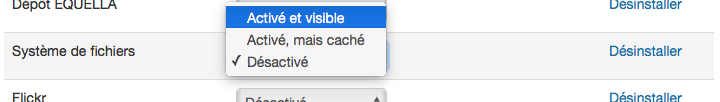
\includegraphics[width=13cm]{repo-filesystem-usb-1.png}
\end{minipage}
\end{figure}

Click on \emph{Save}.
Then, on the same row, click on \emph{Settings}, then on \emph{Create a repository instance}.
Finally select \emph{usb} from the drop-down menu, and enter \emph{USB Drives} in the mandatory \emph{Name} field.
\begin{figure}[!ht]
\begin{minipage}[b]{\linewidth}\centering
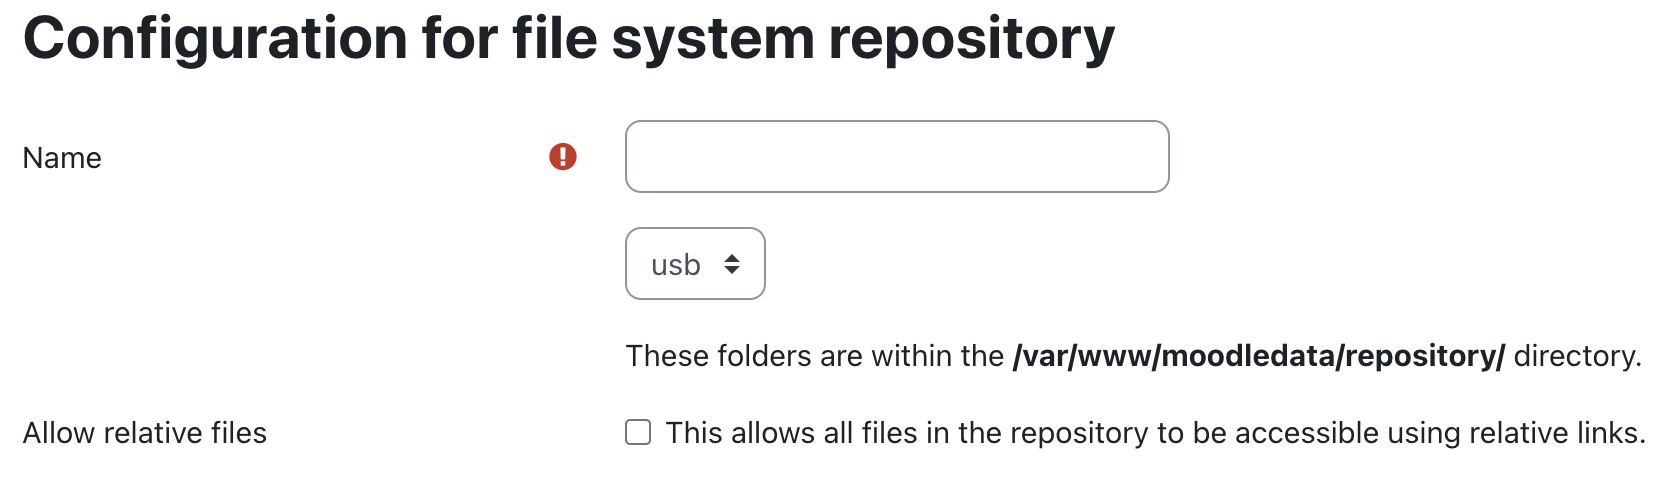
\includegraphics[width=13cm]{repo-filesystem-usb-2.png}
\end{minipage}
\end{figure}

\subsection{SFTP upload}

We create a directory in which the files will be dropped in order to be accessible from Moodle, as well as a link to the Moodle data directory.
Appropriate permissions and ownership are set on this directory, including SGID permission.

\begin{lstlisting}[language=bash]
$ mkdir -p /home/moodlebox/files
$ sudo chown -R moodlebox:www-data files/
$ sudo chmod g+s files/
$ sudo ln -s /home/moodlebox/files /var/www/moodledata/repository
\end{lstlisting}

The repository is then configured in a similar way to the \textsl{USB Drive} repository above, by specifying the directory \emph{files} and enter \emph{SFTP Documents} as the repository name.

If the main username of the MoodleBox is changed, the soft link will be broken.
To prevent this issue, we check the link at login time and fix it if needed, by adding the following lines to file \lstinline{/home/moodlebox/.profile}.

\begin{lstlisting}[language=bash]
# Fix soft link to repository if broken
SOFTLINK="/var/www/moodledata/repository/files"
if [ ! -e ${SOFTLINK} ] ; then
    rm -f ${SOFTLINK}
    ln -s /home/$(getent passwd 1000 | cut -d: -f1)/files ${SOFTLINK}
fi
\end{lstlisting}

To use the SFTP upload feature, MoodleBox's admin will log in to the MoodleBox using a SFTP software\footnote{For instance: \href{https://filezilla-project.org/}{FileZilla}, \href{https://cyberduck.io/}{Cyberduck}, \href{http://winscp.net/}{WinSCP}.}, with their usual credentials.
They can then upload files in the \lstinline{files} directory.

\section{Additional Moodle configurations}

\subsection{Enable MoodleBox access via the Moodle mobile app}

After logging in to Moodle with the administrator account, we visit \textsl{Site Administration > Advanced features}.
We check the box \emph{Enable web services for mobile devices} and save the changes.

For MoodleBox, which is not intended to be published on the Internet, the warning\footnote{Text of the warning: \textsl{It is recommended to enable HTTPS with a valid certificate. The Moodle app will always try to use a secured connection first}.} about the SSL certificate can be safely ignored.

\iffalse
\begin{verification}
From a smartphone connected to the MoodleBox network via Wi-Fi, launch the Moodle mobile app and connect to the platform using the URL \url{http://moodlebox.home}, with the administrator account.
No errors should be notified, and the dashboard should be displayed on the smartphone screen.
\end{verification}
\fi

\subsection{Install MathJax locally}

By default, Moodle loads the MathJax library from the Internet.
We want that this library is available locally, since MoodleBox is offline most of the time.

We install the MathJax library with Git at the correct location; we get the version supported by Moodle, in a shallow clone to save space, and we set the adequate permissions and ownership.
\begin{lstlisting}[language=bash]
$ sudo git clone --depth=1 -b 2.7.9 https://github.com/mathjax/MathJax.git /var/www/moodle/lib/MathJax
$ sudo chown -R www-data:moodlebox /var/www/moodle/lib/MathJax
$ sudo chmod -R ug+w,o-w /var/www/moodle/lib/MathJax
\end{lstlisting}

We can now update the MathJax library URL in \emph{Site administration > Plugins > Filters > MathJax}, setting it to \lstinline{/lib/MathJax/MathJax.js}.

\subsection{Install utilities for PDF files manipulation in Moodle}

We install Ghostscript and Poppler to enable Moodle to manage PDF annotations and PDF to PNG conversions.
\begin{lstlisting}[language=bash]
$ sudo apt install -y ghostscript poppler-utils
\end{lstlisting}

\subsection{Set Moodle system paths}

We configure the Moodle system paths relevant for the MoodleBox, by visiting \emph{Site administration > Server > System paths}, and we set there the following paths:
\begin{itemize}
\item Path to PHP CLI: \texttt{/usr/bin/php}
\item Path to du: \texttt{/usr/bin/du}
\item Path to ghostscript: \texttt{/usr/bin/gs}
\item Path to pdftoppm: \texttt{/usr/bin/pdftoppm}
\item Path to Python: \texttt{/usr/bin/python}
\end{itemize}

\subsection{Download H5P libraries}

To be able to use H5P out of the box without needing to connect to Internet, we download all the H5P libraries within Moodle user interface, by visiting \emph{Site administration > General > H5P > H5P overview} and click \emph{Run now} under \emph{H5P scheduled task}.

The download time is rather long (around 10 minutes) depending on your Internet connection.

\subsection{Make sure to disable Moodle's debug messages display}

We then disable Moodle debug messages display, by visiting \emph{Site administration > Development > Debugging}, making sure that the checkbox \emph{Display debug messages} is unchecked.

\section{Installation of \textsl{AdminerEvo}}

\textsl{AdminerEvo}, successor of Adminer, is a full-featured database management tool written in PHP.
It consists of a single file ready to be deployed to the server.
We install it by downloading it to the adequate location, and set its appropriate permissions.
\begin{lstlisting}[language=bash]
$ sudo wget -qO- https://download.adminerevo.org/latest/adminer/adminer.zip | zcat > /var/www/moodle/adminer.php
$ sudo chown moodlebox:www-data /var/www/moodle/adminer.php
$ sudo chmod -R 664 /var/www/moodle/adminer.php
\end{lstlisting}

To manage the database with \textsl{AdminerEvo}, the interface should be accessed at \url{http://moodlebox.home/adminer.php}.
To log in, use the credentials set at the MariaDB installation, section~\ref{ssec-mariadb}.

\iffalse
\begin{verification}
Browse to URL \url{http://moodlebox.home/adminer.php}.
The Adminer interface should be displayed.
To log in, use usual credentials: by default, username \emph{moodlebox} and password \emph{Moodlebox4\$}.
\end{verification}
\fi

\section{Installation of \texttt{rpi-clone}}

The \texttt{rpi-clone} utility enables to make copies of the currently running MoodleBox image to an external device.
It consists of a single file ready to be deployed to the server.
We install it by downloading it to the adequate location, and set its appropriate permissions.
\begin{lstlisting}[language=bash]
$ wget -c https://raw.githubusercontent.com/geerlingguy/rpi-clone/master/rpi-clone -O /usr/local/sbin/rpi-clone
$ sudo chown root:root /usr/local/sbin/rpi-clone
$ sudo chmod -R 775 /usr/local/sbin/rpi-clone
\end{lstlisting}

Usage of \texttt{rpi-clone} is not covered in this document.

\section{Optimisation}\label{sec-optimisation}

To make the MoodleBox more comfortable to use, it is necessary to take care of its optimisation.
We configure Moodle's cache, as well as its management of file uploads and downloads.

\subsection[Setup RAM disks for specific Moodle directories]{Setup RAM disks for specific Moodle directories\footnote{Partly inspired by \url{https://www.leading-interactive.de/e-learning/moodle-performance-tuning-mit-tmpfs/}.}}

Some files in Moodle data directory are needed very frequently and quickly, e.g. temporary files and session data.
To enable faster access to them, we deliver them directly from the server's RAM, faster than the microSD card, using RAM disks.

RAM disks are also used for the temporary and sessions directories in Moodle.
These two directories are located Moodle data directory \emph{moodledata}.

We define the RAM disks in the Raspberry Pi's mount table.
To do this, we add the following lines to the file \lstinline{/etc/fstab}:
\begin{lstlisting}[language=bash]
tmpfs /var/www/moodledata/temp tmpfs size=64M,mode=775,uid=www-data,gid=www-data 0 0
tmpfs /var/www/moodledata/sessions tmpfs size=16M,mode=775,uid=www-data,gid=www-data 0 0
\end{lstlisting}

%\begin{lstlisting}[language=bash]
%$ sudo nano /etc/fstab
%\end{lstlisting}
%
%Le contenu du fichier \lstinline{/etc/fstab} sera alors :
%\lstinputlisting[language=bash]{files/fstab}

\subsection{Install Redis for caching}

We use Redis to speed up Moodle caching.
Let's install Redis and its PHP module.

\begin{lstlisting}[language=bash]
$ sudo apt install -y redis php-redis
\end{lstlisting}

\subsection{Moodle cache configuration}\label{ssec-cache}

After a reboot of the MoodleBox, the Moodle cache can be configured.

Log in to Moodle with the administrator account, then visit \textsl{Site Administration > Plugins > Caching > Configuration}.
We create one new Redis cache store, by clicking on \emph{Add Instance} in the \emph{Installed cache stores} section (at the top of the page).

\begin{figure}[!ht]
\centering
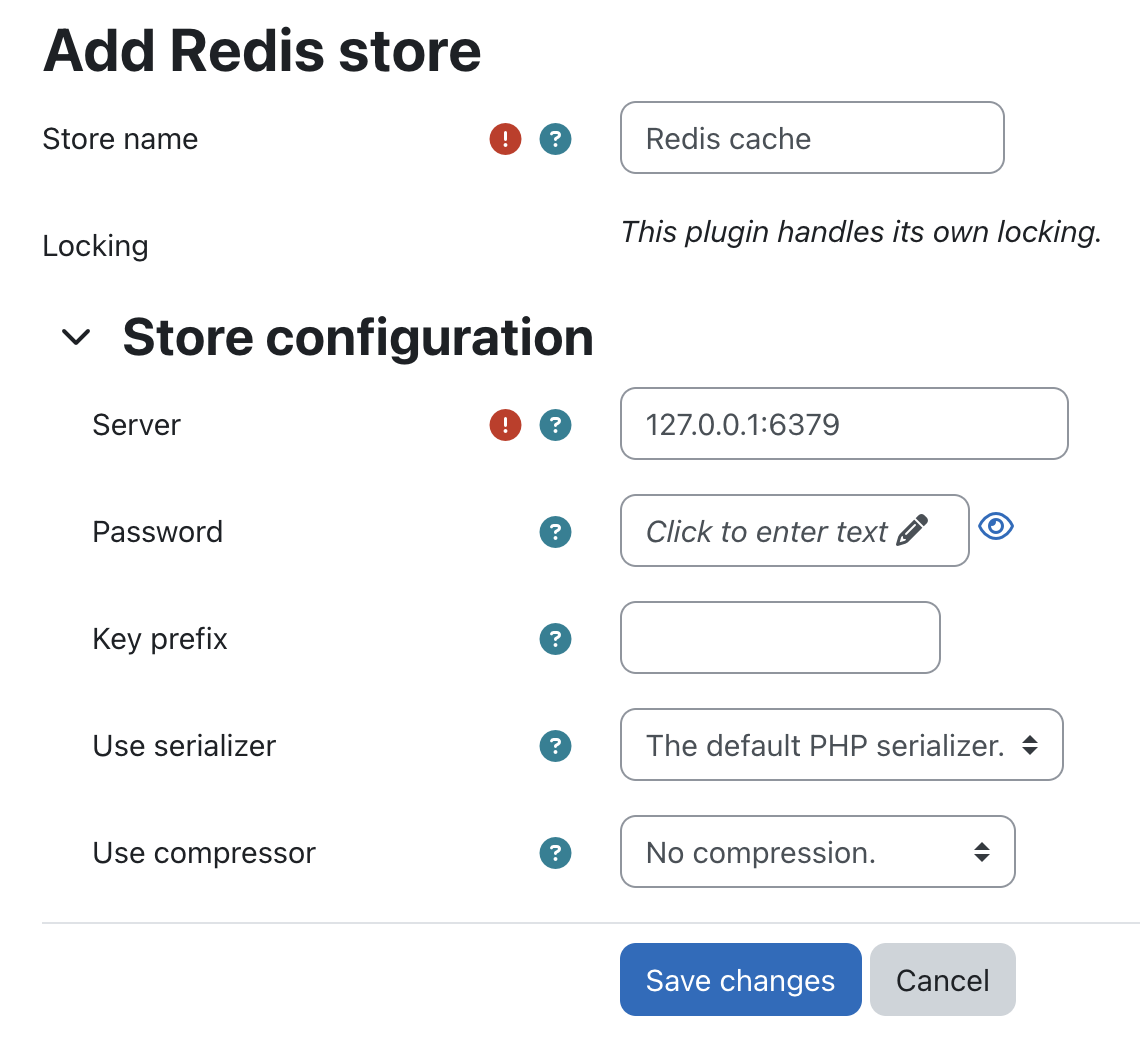
\includegraphics[width=7cm]{cache-redis.png}
\end{figure}

Store name: \emph{Redis cache}, Server: \emph{127.0.0.1:6379}, and we save the changes.

Finally, we map the Application and Session stores to this new cache instance, by clicking on \emph{Edit mappings} in the \emph{Stores used when no mapping is present} section, at the very bottom of the page.
We map there Application and Session to \emph{Redis cache}.

\iffalse
\begin{figure}[!ht]
\begin{minipage}[b]{\linewidth}
\centering
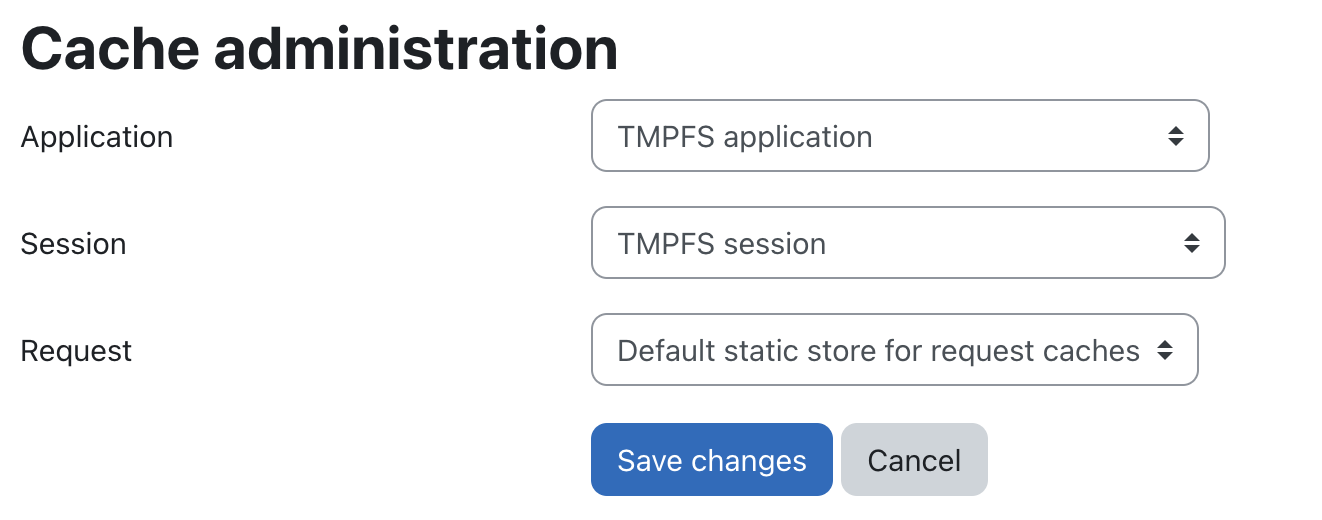
\includegraphics[width=8.5cm]{cache-mappings.png}
\end{minipage}
\end{figure}
\fi

\subsection{MariaDB optimisation}\label{ssec-mariadb-optimisation}

For a better performance, we tweak the value of some MariaDB variables in the file \lstinline{/etc/mysql/mariadb.conf.d/50-server.cnf}:
\begin{lstlisting}[language=bash]
skip-name-resolve
query_cache_size        = 2M
log_error = /var/log/mysql/error.log
\end{lstlisting}

\subsection{PHP optimisation}\label{ssec-php-optimisation}

For a better performance, we tweak the value of a PHP variable in the file \lstinline{/etc/php/8.2/fpm/pool.d/www.conf}:
\begin{lstlisting}[language=bash]
pm.max_requests = 50
\end{lstlisting}

\section{Setup of partition auto-resizing}

This setting is only useful if you intend to distribute a disk image that you'll minimise.
It can be skipped otherwise.

In order to avoid the user having to manually resize the working partition, automatic resizing at first boot can be configured.
The method used is the same than when building the \emph{Raspberry Pi OS Lite} disk image.\footnote{See \url{https://github.com/RPi-Distro/pi-gen}.}

We copy the file \lstinline{resize2fs_once} below into the \lstinline{/etc/init.d/} directory, and give it the appropriate permissions to be launched on reboot.
\lstinputlisting[language=bash]{files/resize2fs_once}

Finally, before the last shutdown before cloning and minimising the disk image, we finish by running the command
\begin{lstlisting}[language=bash]
$ sudo systemctl enable resize2fs_once
\end{lstlisting}
then we add at the end of the unique line of the file \lstinline{/boot/firmware/cmdline.txt} the instruction below, immediately after the text \lstinline{rootwait} (without forgetting a space).
\begin{lstlisting}[language=bash]
quiet init=/usr/lib/raspi-config/init_resize.sh
\end{lstlisting}

It is essential that the MoodleBox is not restarted, otherwise the entire operation described in this section will have to be repeated.

\section{Cleanup}

The commands below will clean up the MoodleBox and reduce the amount of disk space it requires, if you intend distributing it as a disk image.

\begin{lstlisting}[language=bash]
$ sudo rm -rf /var/www/moodledata/temp/*
$ sudo rm -rf /var/www/moodledata/trashdir/*
$ sudo rm -rf /var/www/moodledata/sessions/*
$ sudo rm -rf /var/backups/
$ sudo mysql moodle -e "truncate table moodle.mdl_logstore_standard_log"
$ sudo mysql moodle -e "truncate table moodle.mdl_config_log"
$ sudo mysql moodle -e "truncate table moodle.mdl_upgrade_log"
$ sudo mysql moodle -e "truncate table moodle.mdl_task_log"
$ sudo apt clean
$ sudo rm -rf /var/cache/debconf/*
$ sudo rm -rf /var/lib/apt/lists/*
$ sudo rm -rf /tmp/*
$ sudo rm -rf /var/tmp/*
$ sudo rm -f ~/.mysql_history ~/.nano_history ~/.bash_history
$ sudo apt --purge autoremove
$ sudo truncate -s 0 /root/.bash_history
\end{lstlisting}

\end{document}
%%
%% The end
